\documentclass{beamer}[10]
\usepackage{pgf}
\usepackage[danish]{babel}
\usepackage[utf8x]{inputenc}
\usepackage{beamerthemesplit}
\usepackage{graphics,epsfig, subfigure}
\usepackage{url}
\usepackage{hyperref}
\graphicspath{ {images/} }
\usepackage{parallel}
\usepackage{fixltx2e}
\usepackage{xcolor}

\definecolor{kugreen}{RGB}{0,153,153}
\setbeamercovered{transparent}
\mode<presentation>
\usetheme[numbers,totalnumber,compress,sidebarshades]{PaloAlto}
\setbeamertemplate{footline}[frame number]

  \usecolortheme[named=kugreen]{structure}
  \useinnertheme{circles}
  \usefonttheme[onlymath]{serif}
  \setbeamercovered{transparent}
  \setbeamertemplate{blocks}[rounded][shadow=true]

\logo{\includegraphics[width=0.8cm]{KULogo}}
%\useoutertheme{infolines} 
\title{Security Protocols Checker}
\author{\textbf{Autor}\newline Ștefan Stan}
%\textbf{Coordonator științific} \newline Lect. dr. Cosmin-Nicolae Vârlan
\institute{\normalsize \textbf{Coordonator științific} \newline Lect. dr. Cosmin-Nicolae Vârlan \newline \newline \small Facultatea de Informatică\\ Universitatea Alexandru Ioan Cuza din Iași}
\date{3 Iulie 2015}

\begin{document}
\frame{\titlepage \vspace{-0.5cm}
}

\frame
{
\frametitle{Cuprins}
\tableofcontents
}

\section{Introducere}

\Large
\subsection{Cuvinte cheie}

\frame{
\frametitle{Cuvinte cheie}
\begin{center}
\textcolor{kugreen}{
protocol de securitate, model checking,\\ integritate, confidențialitate,\\
Java, analiză sintactică, analiză semantică}
\end{center}
}
\normalsize

\subsection{Obiective}

\frame{
\frametitle{Obiective}
\begin{itemize}
\item definirea, încărcarea în memorie și rularea protocoalelor de securitate descrise la nivel teoretic;
\item verificarea automată a proprietăților de securitate:
\begin{itemize}
\vspace{0.1cm}
\item \textbf{Integritate}
\\
protecția informației spre a nu fi \textbf{modificată} de către surse neautorizate;
\vspace{0.3cm}
\item \textbf{Confidențialitate}
\\
protecția informației spre a nu fi \textbf{accesată} de către surse neautorizate.
\end{itemize}
\end{itemize}
}

\subsection{Aplicații similare}

\frame{
\frametitle{Aplicații similare}
\textbf{Scyther}
\newline
\begin{itemize}
\item Cas Cremers - \textit{Scyther - Semantics and Verification of Security Protocols}
\vspace{0.15cm}
\item Verifică \textbf{integritatea} și \textbf{confidențialitatea} unei instanțe de protocol
\vspace{0.15cm}
\item Arată atacurile posibile în manieră grafică
\end{itemize}
}

\section{Modelare Teoretică}

\subsection{Sursa de inspirație}
\frame{
\frametitle{Sursa de inspirație}

\begin{columns}
\column{0.62\textwidth}

\small
\textbf{Reasoning about minimal anonymity in security protocols}
\newline
\newline
Autori:
\begin{itemize}
\item Prof. dr. Ferucio Laurenţiu Ţiplea
\item Lect. dr. Cosmin Vârlan
\item Loredana Vamanu
\end{itemize}
\column{0.45\textwidth}
\begin{figure}
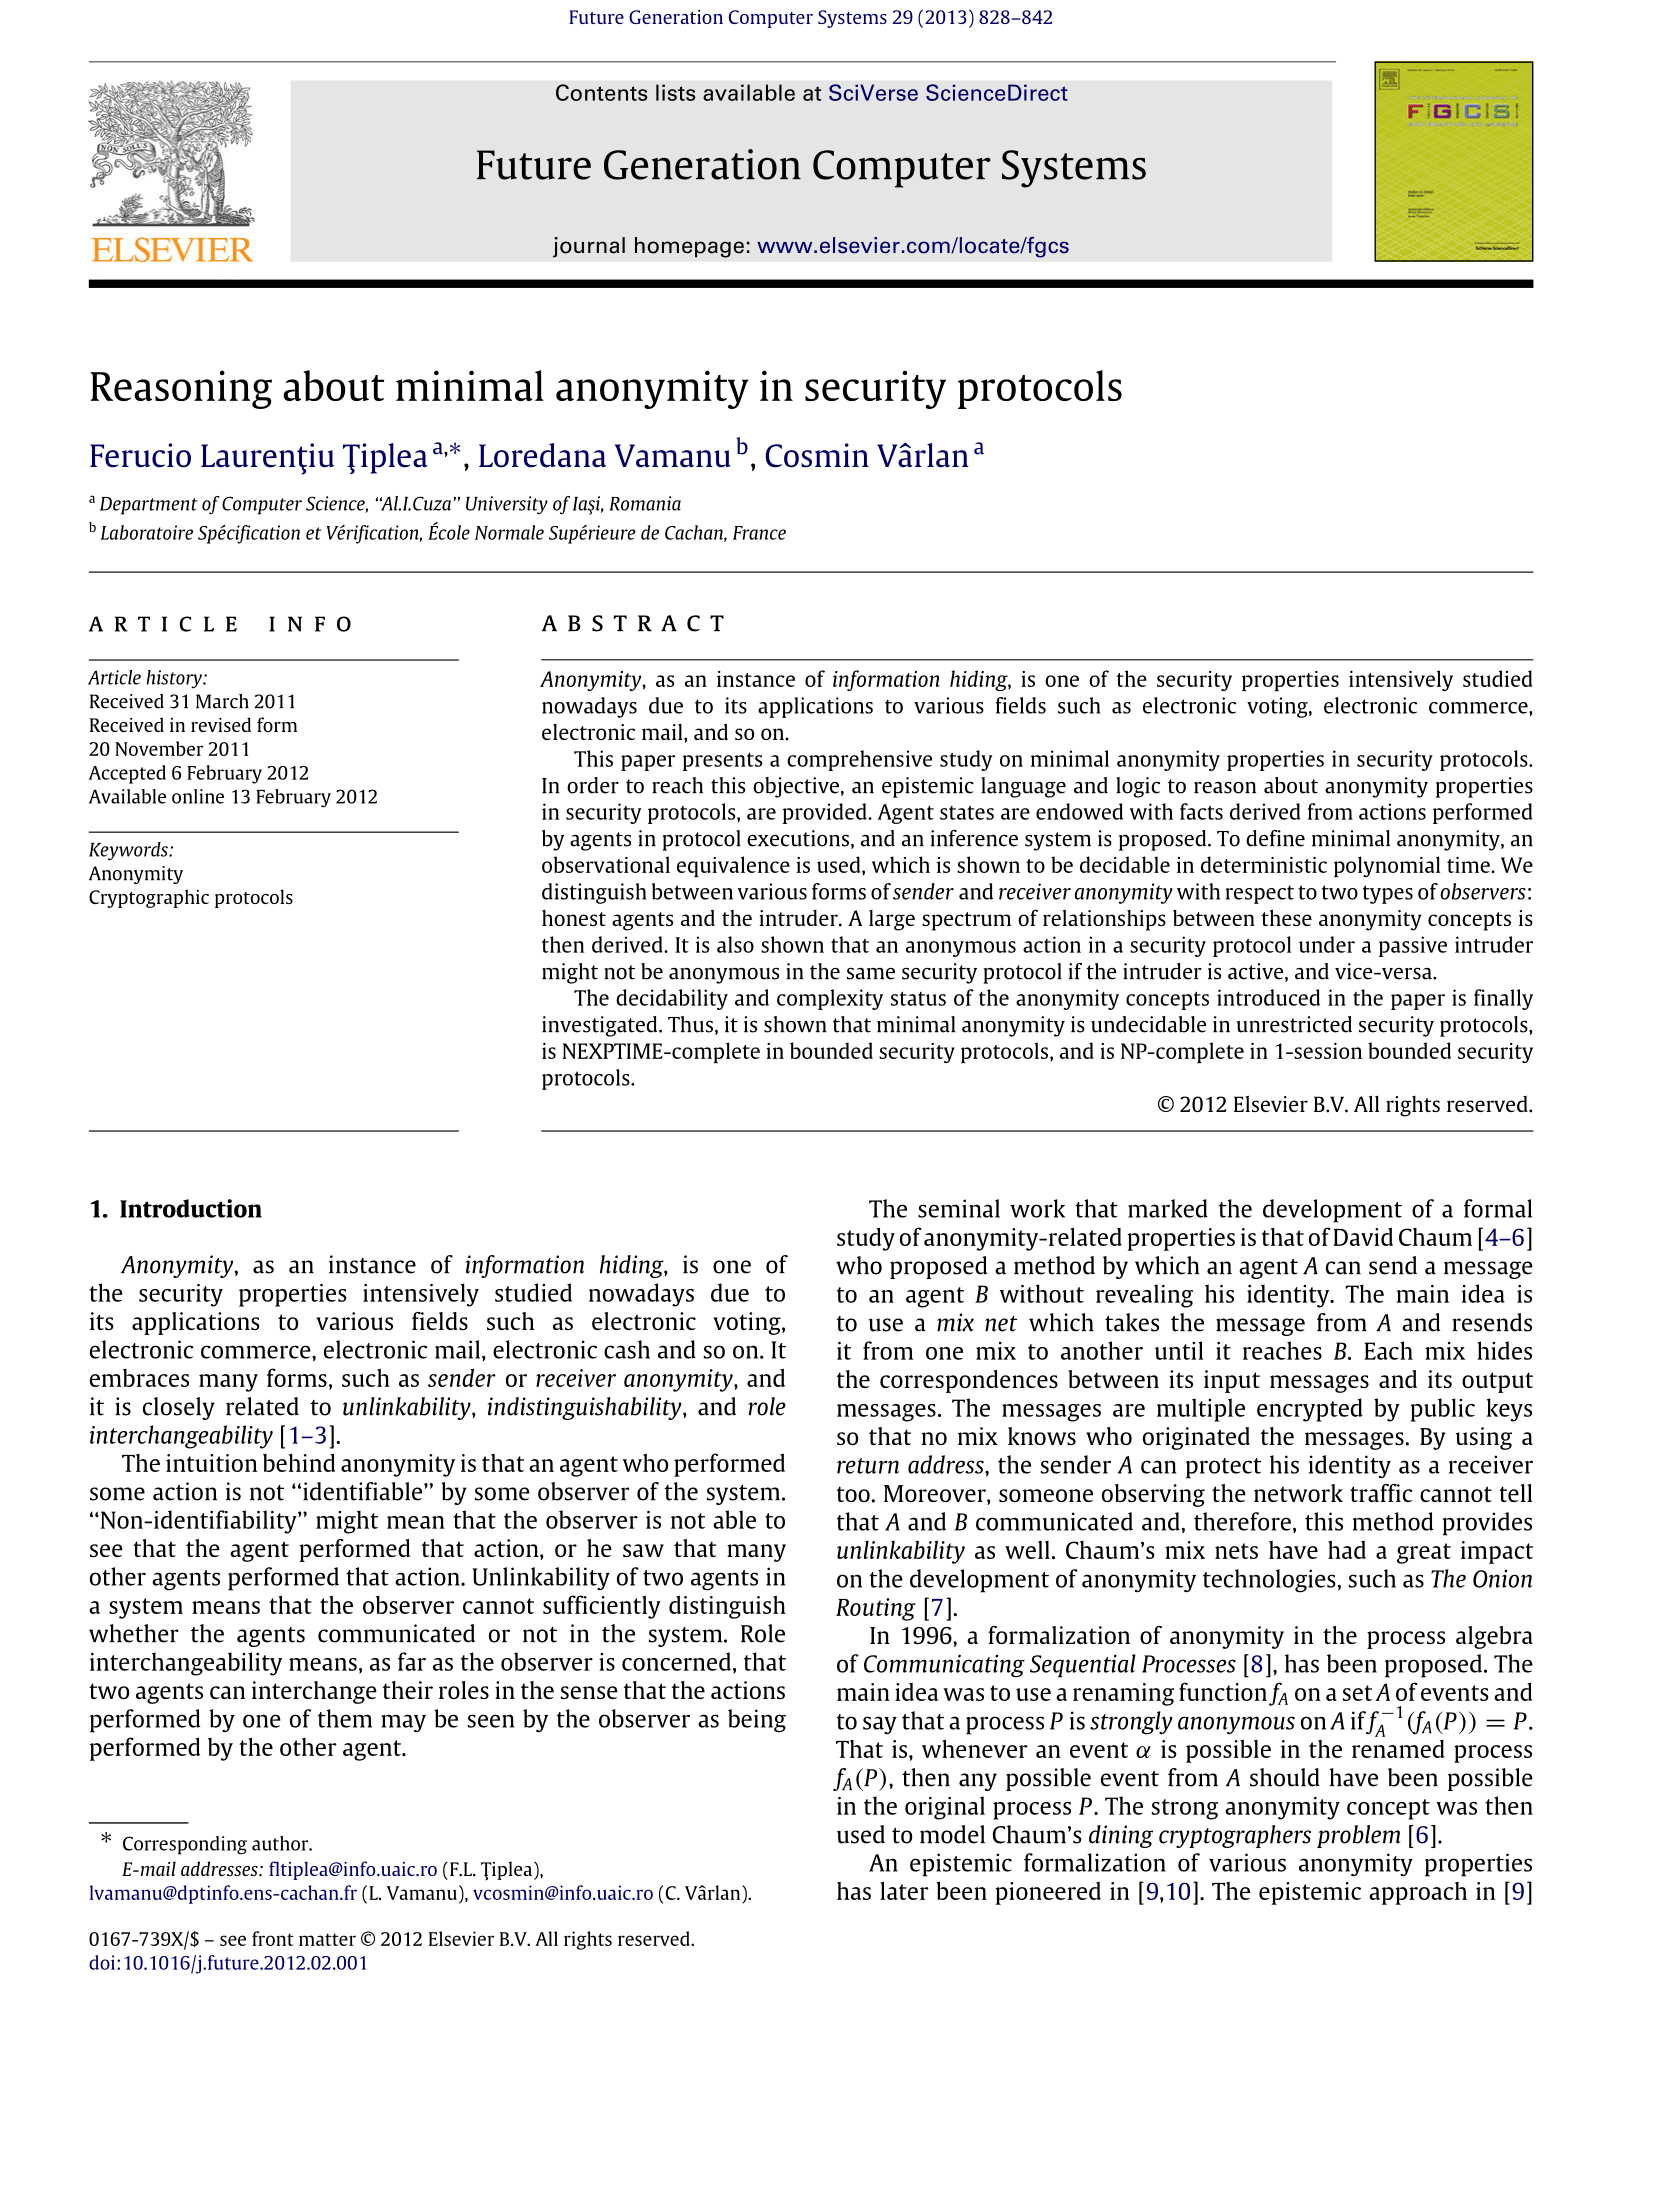
\includegraphics[scale=0.11]{FGCS}
\end{figure}

\end{columns}

%\vspace{3cm}
}

\subsection{Protocoale de securitate}
\frame{
\frametitle{Protocoale de securitate}
\par
\textcolor{kugreen}{Signatura unui protocol - $\mathcal{S = (A, K, N)}$}
\vspace{0.125cm}
\newline
$\mathcal{A}$ - mulțime finită de \textit{agenţi}; include \textit{intrusul} - \textit{I}
\newline
$\mathcal{K}$, $\mathcal{N}$ - două mulţimi cel mult numărabile de \textit{chei} şi, respectiv, \textit{nonce}-uri.
\vspace{0.6cm}
\newline
\textcolor{kugreen}{Termi}
\vspace{0.125cm}
\newline
$\mathcal{T}_{0}$ = $\mathcal{A}$ $\cup$ $\mathcal{K}$ $\cup$ $\mathcal{N}$ - Mulţimea termilor de bază
\newline
Mulţimea $\mathcal{T}$ a termilor este definită inductiv:
\setbeamertemplate{itemize items}[triangle]
\begin{itemize}
  \item $\mathcal{T}_{0}$ $\in$ $\mathcal{T}$;
  \item t$_{1}$, t$_{2}$ $\in$ $\mathcal{T}$ $\Rightarrow$ (\textit{t$_{1}$}, \textit{t$_{2}$}) $\in$ $\mathcal{T}$;
  \\ (\textit{t$_{1}$}, ..., \textit{t$_{n}$}) = ((\textit{t$_{1}$}, ..., \textit{t$_{n-1}$}) \textit{t$_{n}$}) $\Rightarrow$ (\textit{t$_{1}$}, ..., \textit{t$_{n}$}) $\in$ $\mathcal{T}$, n$\geq$3; 
  \item \textit{t} $\in$ $\mathcal{T}$, \textit{K} $\in$ $\mathcal{K}$ $\Rightarrow$ \{\textit{t}\}\textsubscript{\textit{K}} $\in$ $\mathcal{T}$;
  \end{itemize}
}

\section{Implementare}

\subsection{Arhitectura aplicației}

\frame{
\frametitle{Arhitectura aplicației}
\begin{figure}[h]
	\centering
    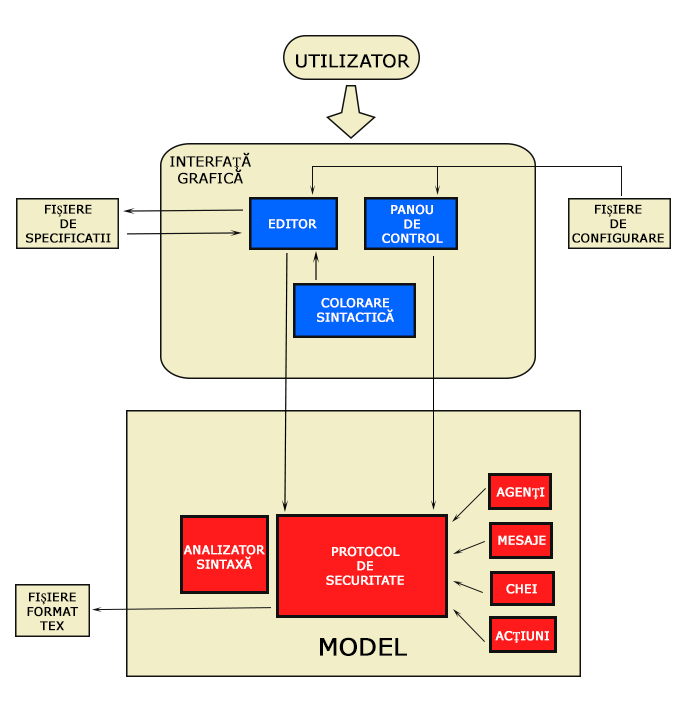
\includegraphics[scale=0.3]{diagram}
\end{figure}
}

\subsection{Descrierea unui protocol}

\frame{
\frametitle{Descrierea unui protocol}
\textcolor{kugreen}{\textbf{Definirea specificației}}
\vspace{0.075cm}
\\
agent$_{1}$ : IK { info$_{11}$, $\ldots$, info$_{1m}$}
\\
$\ldots$
\\
agent$_{n}$ : IK { info$_{n1}$, $\ldots$, info$_{np}$}
\vspace{0.18cm}
\\
acțiune$_{1}$
\\
$\ldots$
\\
acțiune$_{k}$
\vspace{0.18cm}
\\
\textcolor{kugreen}{\textbf{Informație}}
\vspace{0.075cm}
\\
agent$\vert$ticket$\vert$nonce$\vert$cheie
\vspace{0.18cm}
\\
\textcolor{kugreen}{\textbf{Acțiune}}
\vspace{0.075cm}
\\
agent$_{1}$ ! agent$_{2}$ : (termiGenerați) mesaj
\\
agent$_{1}$ ? agent$_{2}$ : mesaj
}
\iffalse
\subsection{Funcționalități importante}

\frame{
\frametitle{Funcționalități importante}
\textbf{Verificarea sintactică} este realizată de un analizator sintactic descendent generat de utilitarul Java Compiler Compiler. Acesta folosește o gramatică \textbf{\textit{LL(k)}} ce descrie limbajul dorit.
\vspace{0.25cm}
\\
\textbf{Verificarea semantică} se folosește pentru a valida cunoștințele agenților (cheile publice cunoscute de toți agenții, cheile private doar de agentul descris de cheie etc.).
\vspace{0.25cm}
\\
\textbf{Colorarea sintactică} a specificației - împărțirea în tokeni și colorarea conform fișierului de configurare \texttt{colors.css}.
\vspace{0.25cm}
}

\subsection{Algoritmul de verificare}

\frame{
\frametitle{Verificarea proprietăților de securitate}
\textbf{Identitatea instanțelor clasei \texttt{Term}}
\\
Metodele \texttt{theSame()} și \texttt{equals()}.
\vspace{0.375cm}
\\
\textbf{Metode de atac}
\\
Atacatorul poate modifica un mesaj transmis între doi agenți. Metoda \texttt{replaceMessage()} a clasei \texttt{Intruder}.
\vspace{0.375cm}
\\
\textbf{Algoritmul de verificare}
\begin{itemize}
\item Crearea și rularea instanței ajutătoare;
\item Crearea instanței de test;
\item Rularea algoritmului de verificare pe instanța de test.
\end{itemize}
}

\subsection{Modelare și proiectare}

\frame{
\frametitle{Șabloane de proiectare}
\pause
\textbf{Composite}
\\
Orice term de bază este term și orice term compus este term. Termii compuși sunt reprezentați prin intermediul unor structuri arborescente care pot fi manevrate la fel ca și termii de bază.
\vspace{0.375cm}
\\
\pause
\textbf{Singleton}
\\
Existența, la un moment dat, a unui singur atacator, accesibil de oriunde.
\vspace{0.375cm}
\\
\pause
\textbf{Model-View-Controller}
\\
Aplicația a fost împărțită în module ușor manevrabile și la care se putea lucra într-un mod independent.
}
\fi


\section{Exemplu de rulare}

\frame{
\frametitle{Descrierea specificației protocolului}
\hspace{3.2cm}
Specificație protocol:
\vspace{0.5cm}
\\
\hspace{2.7cm}
\textit{A} ! \textit{B} \hspace{1.3 mm}: (\{\textit{N}\textsubscript{1\textsubscript{A}}\}) \{\textit{N}\textsubscript{1\textsubscript{A}}\}\textit{K}\rlap{\textsuperscript{\textit{e}}}\textsubscript{B}\\
\vspace{0.15cm}
\hspace{2.7cm}
\textit{B} ? \textit{A} : \{\textit{N}\textsubscript{1\textsubscript{A}}\}\textit{K}\rlap{\textsuperscript{\textit{e}}}\textsubscript{B}\\
\vspace{0.15cm}
\hspace{2.7cm}
\textit{B} ! \textit{A} \hspace{1.3 mm}: \{\textit{N}\textsubscript{1\textsubscript{A}}\}\textit{K}\rlap{\textsuperscript{\textit{e}}}\textsubscript{A}\\
\vspace{0.15cm}
\hspace{2.7cm}
\textit{A} ? \textit{B} : \{\textit{N}\textsubscript{1\textsubscript{A}}\}\textit{K}\rlap{\textsuperscript{\textit{e}}}\textsubscript{A}
}

\subsection{Rulare - Security Protocols Checker}
\frame{
\frametitle{Rulare - Security Protocols Checker}

Agenți comuni celor două instanțe de protocol: \textit{B}
\newline
\begin{Parallel}[v]{0.48\textwidth}{0.48\textwidth}
\ParallelLText{\noindent
------------Instanța 1------------\newline 
\newline 
\textit{A} ! \textit{B} \hspace{1.3 mm}: (\{\textit{N}\textsubscript{1\textsubscript{A}}\}) \{\textit{N}\textsubscript{1\textsubscript{A}}\}\textit{K}\rlap{\textsuperscript{\textit{e}}}\textsubscript{B}\newline 
\textit{A} generated \{\textit{N}\textsubscript{1\textsubscript{A}}\} for \textit{B}\newline 
\textit{A} sent \{\textit{N}\textsubscript{1\textsubscript{A}}\}\textit{K}\rlap{\textsuperscript{\textit{e}}}\textsubscript{B} to \textit{B}\newline 
\textit{I} received \{\textit{N}\textsubscript{1\textsubscript{A}}\}\textit{K}\rlap{\textsuperscript{\textit{e}}}\textsubscript{B}\newline 
\newline 
\newline
\newline
\newline
\textit{B} ? \textit{A} : \{\textit{N}\textsubscript{1\textsubscript{A}}\}\textit{K}\rlap{\textsuperscript{\textit{e}}}\textsubscript{B}\newline 
\textit{B} received \{\textit{N}\textsubscript{1\textsubscript{A}}\}\textit{K}\rlap{\textsuperscript{\textit{e}}}\textsubscript{B} from \textit{A}\newline 
\textit{B} received \textit{N}\textsubscript{1\textsubscript{A}} from \textit{A}\newline 
\newline 
}
\ParallelRText{\noindent
------------Instanța 2------------\newline 
\newline 
\textit{I}!\textit{B}:\{\textit{N}\textsubscript{1\textsubscript{A}}\}\textit{K}\rlap{\textsuperscript{\textit{e}}}\textsubscript{B}\newline 
I trimite același mesaj care s-a trimis în instanța numărul 1, în aceeași acțiune.\newline 
                Deoarece mai tarziu va descoperi [\textit{N}\textsubscript{1\textsubscript{A}}] din cealaltă instanță de protocol\newline 
\newline\textit{B}?\textit{I}:\{\textit{N}\textsubscript{1\textsubscript{A}}\}\textit{K}\rlap{\textsuperscript{\textit{e}}}\textsubscript{B}\newline 
\textit{B} received \{\textit{N}\textsubscript{1\textsubscript{A}}\}\textit{K}\rlap{\textsuperscript{\textit{e}}}\textsubscript{B} from \textit{I}\newline 
\textit{B} received \textit{N}\textsubscript{1\textsubscript{A}} from \textit{I}\newline 
}
\ParallelPar
\end{Parallel}
}

\frame{
\frametitle{Rulare - Security Protocols Checker}

\begin{Parallel}[v]{0.48\textwidth}{0.48\textwidth}
\ParallelLText{\noindent
\newline
\textit{B} ! \textit{A} \hspace{1.3 mm}: \{\textit{N}\textsubscript{1\textsubscript{A}}\}\textit{K}\rlap{\textsuperscript{\textit{e}}}\textsubscript{A}\newline 
\textit{B} sent \{\textit{N}\textsubscript{1\textsubscript{A}}\}\textit{K}\rlap{\textsuperscript{\textit{e}}}\textsubscript{A} to \textit{A}\newline 
\textit{I} received \{\textit{N}\textsubscript{1\textsubscript{A}}\}\textit{K}\rlap{\textsuperscript{\textit{e}}}\textsubscript{A}\newline 
\newline 
\textit{A} ? \textit{B} : \{\textit{N}\textsubscript{1\textsubscript{A}}\}\textit{K}\rlap{\textsuperscript{\textit{e}}}\textsubscript{A}\newline 
\textit{A} received \{\textit{N}\textsubscript{1\textsubscript{A}}\}\textit{K}\rlap{\textsuperscript{\textit{e}}}\textsubscript{A} from \textit{B}\newline 
\textit{A} received \textit{N}\textsubscript{1\textsubscript{A}} from \textit{B}\newline 
\newline 
}
\ParallelRText{\noindent
\newline
\textit{B}!\textit{I}:\{\textit{N}\textsubscript{1\textsubscript{A}}\}\textit{K}\rlap{\textsuperscript{\textit{e}}}\textsubscript{I}\newline 
\textit{B} sent \{\textit{N}\textsubscript{1\textsubscript{A}}\}\textit{K}\rlap{\textsuperscript{\textit{e}}}\textsubscript{I} to \textit{I}\newline 
\textit{I} received \{\textit{N}\textsubscript{1\textsubscript{A}}\}\textit{K}\rlap{\textsuperscript{\textit{e}}}\textsubscript{I}\newline 
\newline\textit{I}?\textit{B}:\{\textit{N}\textsubscript{1\textsubscript{A}}\}\textit{K}\rlap{\textsuperscript{\textit{e}}}\textsubscript{I}\newline 
\textit{I} received \{\textit{N}\textsubscript{1\textsubscript{A}}\}\textit{K}\rlap{\textsuperscript{\textit{e}}}\textsubscript{I} from \textit{B}\newline 
\textcolor{red}{\textit{I} received \textit{N}\textsubscript{1\textsubscript{A}} from \textit{B}}\newline 
\newline
}
\ParallelPar
\end{Parallel}
}

\subsection{Rulare - Scyther}

\frame{
\frametitle{Rulare - Scyther}
\begin{figure}[h]
	\centering
    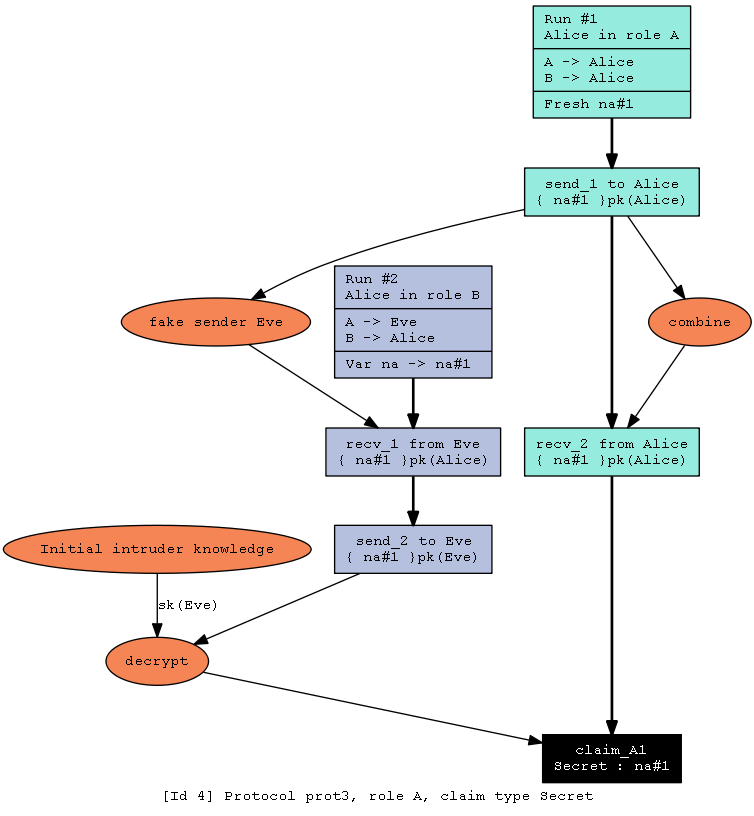
\includegraphics[scale=0.325]{little}
\end{figure}
}

\frame{
\frametitle{Corectarea specificației}
\hspace{3.2cm}
Specificație corectă:
\vspace{0.5cm}
\\
\hspace{2.7cm}
\textit{A} ! \textit{B} \hspace{1.3 mm}: (\{\textit{N}\textsubscript{1\textsubscript{A}}\}) \{\textcolor{red}{A},\textit{N}\textsubscript{1\textsubscript{A}}\}\textit{K}\rlap{\textsuperscript{\textit{e}}}\textsubscript{B}\\
\vspace{0.15cm}
\hspace{2.7cm}
\textit{B} ? \textit{A} : \{\textcolor{red}{A},\textit{N}\textsubscript{1\textsubscript{A}}\}\textit{K}\rlap{\textsuperscript{\textit{e}}}\textsubscript{B}\\
\vspace{0.15cm}
\hspace{2.7cm}
\textit{B} ! \textit{A} \hspace{1.3 mm}: \{\textit{N}\textsubscript{1\textsubscript{A}}\}\textit{K}\rlap{\textsuperscript{\textit{e}}}\textsubscript{A}\\
\vspace{0.15cm}
\hspace{2.7cm}
\textit{A} ? \textit{B} : \{\textit{N}\textsubscript{1\textsubscript{A}}\}\textit{K}\rlap{\textsuperscript{\textit{e}}}\textsubscript{A}
}

\section{Concluzii}

\frame{
\frametitle{Concluzii}
\begin{itemize}
\item Utilitar ce încarcă în memorie și rulează protocoale de securitate descrise în fișiere de specificație;
\item Ofera mijloacele necesare pentru verificarea \textbf{integrității} și a \textbf{confidențialității};
\item Verifică dacă, la nivel teoretic, proprietățile sunt asigurate de către un protocol;
\end{itemize}
}

\end{document}
